\section{Cameras}

In graphics, a camera projects a 3D scene onto a 2D plane which
can be displayed on a screen. If we model the camera as a point,
then the problem becomes a linear algebra issue of projecting a
set of points onto a plane determined by the camera. We must
display only surfaces not obscured by other surfaces, not accounting
for things like transparency.

The camera is a grid of pixels and an eye. The eye shoots out rays
to the scene and where those rays intersect the plane, draws a point.

\begin{figure}
    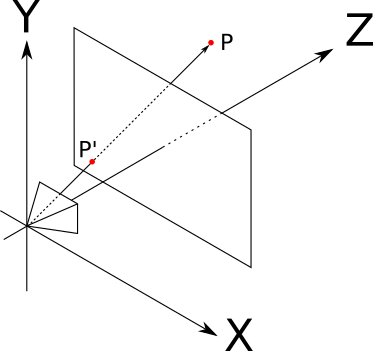
\includegraphics{images/camera.png}
    \caption{Camera}
    \label{fig:camera}
\end{figure}

A \emph{pose} consists of three translations and three rotations.
Setting each results in a unique camera pose in 3D space.

\marginnote{There are several ways to approximate the way the human
    eye sees, the method used in this class is called the planar pinhole method.
    There are many, many other camera models, for instance thin lens camera,
    orthographic camera, spherical camera, fisheye camera.}

The issue of projecting a point onto a plane involves linear algebra.
There are known formulas for it, which are not listed here.

The probability that a ray exactly intersects the center of a
pixel is zero.
\marginnote{The probability that a ray exactly intersects the center of a
    pixel is not zero, since floating point numbers have a finite range of
    values they can take, but practically it is zero.}
This means we have to calculate the pixel center closest to the
intersection and use that instead.

The human eye has the wonderful property that it sees things far away
in a panorama, and things that are in close in intricate detail.

Translations of the camera must be with respect to its current orientation.
That is, the camera must move left or right relative to what it sees,
which is more difficult than just changing the x coordinate.